\documentclass[12pt,a4paper,english,oneside,parskip=false]{scrartcl} %parskip=half
\usepackage[T1]{fontenc}
\usepackage[utf8]{inputenc}
\usepackage[english]{babel}

\usepackage{helvet}
\usepackage{amsmath}
\usepackage{amsfonts}
\usepackage{amssymb}

%\usepackage[a4paper, top=20mm, bottom=25mm, left=23mm, right=23mm]{geometry}

\usepackage{mathpazo}

\usepackage{hyphenat}
\usepackage{url}
\usepackage{hyperref}
\hypersetup{%
	final=true,%
	colorlinks=true,%
	linkcolor=black,%
	citecolor=black,%
	urlcolor=black,%
}
\usepackage[babel=true]{csquotes}
\usepackage{graphicx}

%\usepackage{todonotes}

\renewcommand{\familydefault}{\sfdefault}
\fontfamily{phv}\selectfont

\linespread{1.05}
%\setkomafont{disposition}{\sfdefault}
\clubpenalty = 20000
\widowpenalty = 20000

\addto\extrasenglish{%
	\renewcommand{\sectionautorefname}{Section}
	\renewcommand{\subsectionautorefname}{Section}
	\renewcommand{\subsubsectionautorefname}{Section}
}


\begin{document}

\title{Installing OceanTEA with\\Docker Machine on Mac OS X}
%\author{Arne Johanson}
\date{}

\maketitle

\section{Installing Docker Toolbox} \label{sec:docker}

First, you need to install and configure Docker Toolbox: 
\begin{enumerate}
	\item Download the latest version of Docker Toolbox for Mac OS X from:\\ \url{https://www.docker.com/products/docker-toolbox}
	\item Execute the setup program to install Docker Toolbox with default settings.
	\item Execute the \enquote{Docker Quickstart Terminal} in your applications directory:\\
	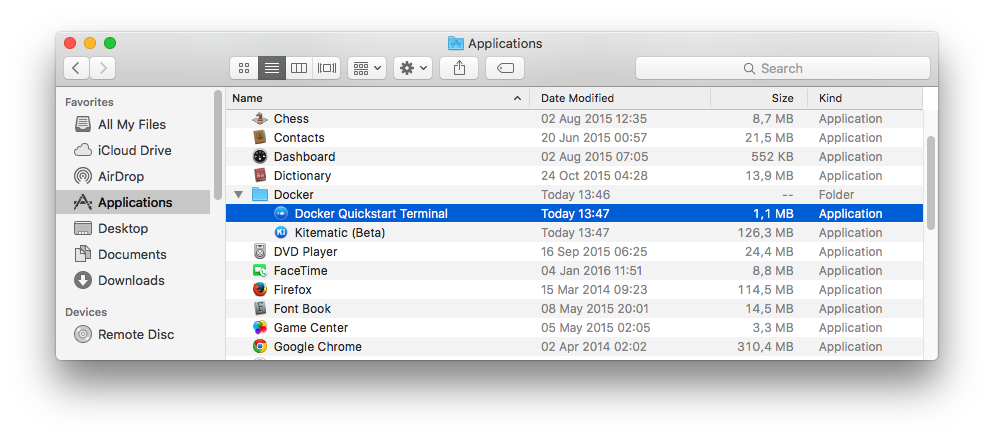
\includegraphics[width=\linewidth]{fig/start_docker_machine}
	\item Wait until the terminal window looks like this:\\
	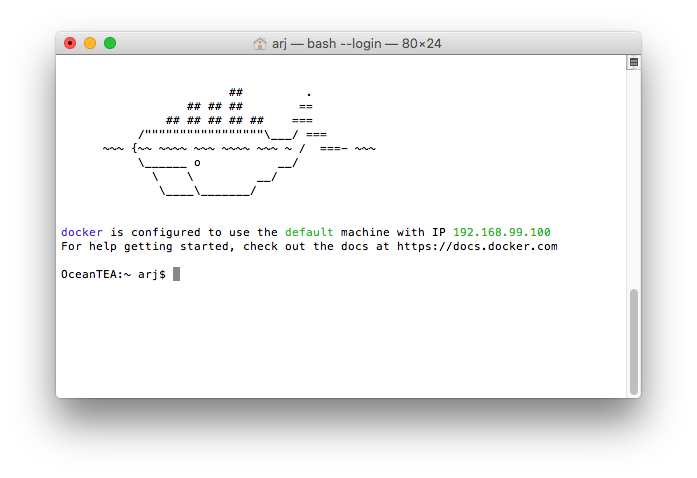
\includegraphics[width=\linewidth]{fig/docker_machine}
	\item Close the terminal window.
\end{enumerate}


\section{Installing Git} \label{sec:git}

The second step is to install Git: 
\begin{enumerate}
	\item Download the latest version of Git for Mac OS X from:\\ \url{https://git-scm.com/download/mac}
	\item Execute the setup program to install Git with default settings. 
\end{enumerate}


\section{Installing OceanTEA} \label{sec:oceantea}

After having installed Docker Toolbox and Git, you can install OceanTEA as follows:
\begin{enumerate}
	\item Download the ZIP archive \texttt{oceantea.zip} from:\\
	\url{https://github.com/a-johanson/oceantea/raw/master/install/docker-local/mac/oceantea.zip}
	\item Extract the archive to any folder you have write access to (e.g., your Desktop). 
	Depending on which web browser you use, the archive might already have been extracted to your Download directory for you. 
	\item Open the Terminal utility:\\
	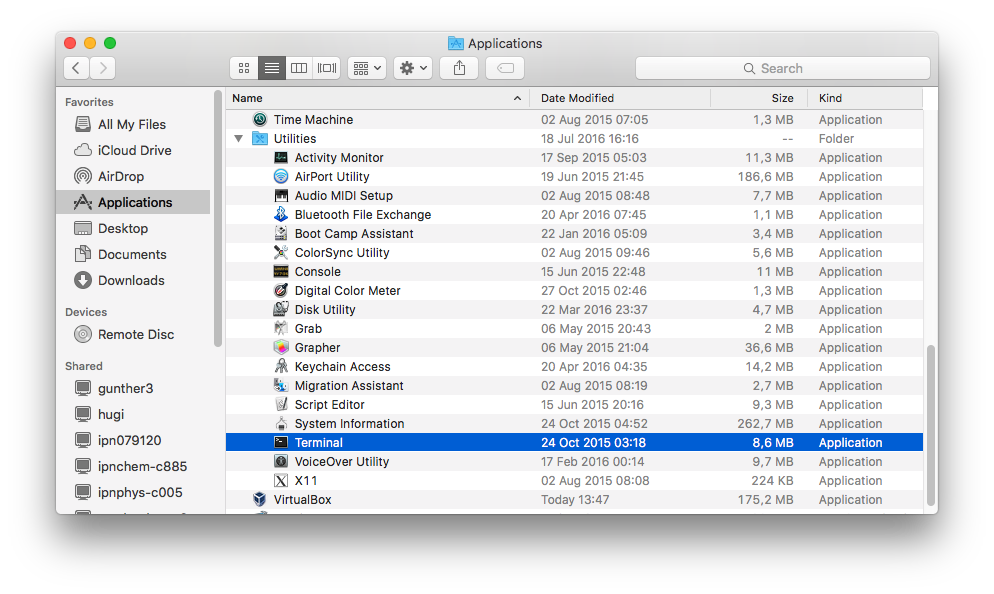
\includegraphics[width=\linewidth]{fig/start_terminal}
	\item Navigate to the folder in which the extracted files from \texttt{oceantea.zip} reside by executing the command:\\
	\texttt{cd path/to/folder}
	\item Mark the scripts contained in that folder as executable:\\
	\texttt{chmod a+x start\_oceantea.sh stop\_oceantea.sh}
	\item Run \texttt{start\_oceantea.sh}:\\
	\texttt{./start\_oceantea.sh}\\
	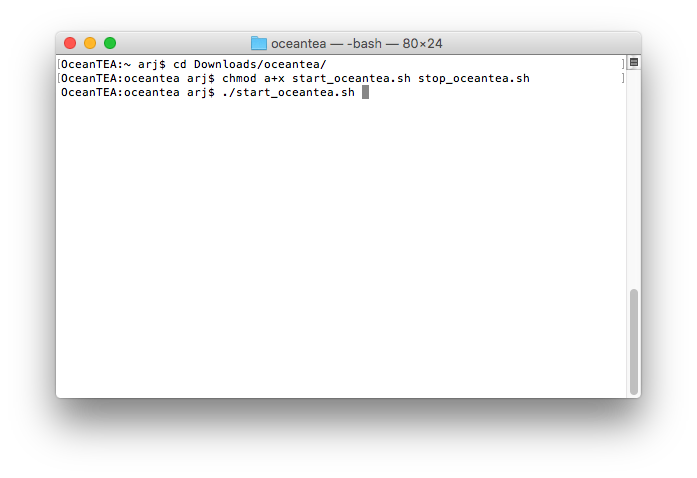
\includegraphics[width=\linewidth]{fig/terminal_input}
	\item Wait for the installation process to complete. After it finishes, your default web browser should open displaying the OceanTEA user interface. 
	To start or stop OceanTEA, execute \texttt{start\_oceantea.sh} or \texttt{stop\_oceantea.sh}, respectively.
\end{enumerate}


\end{document}
